\documentclass[10pt,wide]{mwart}
\usepackage{amsfonts}
\usepackage{amssymb}
\usepackage{graphicx}
\usepackage{svg}
\usepackage[utf8]{inputenc}
\usepackage{tikz}
\usepackage{tabularx}
\usepackage[centertags]{amsmath}
\usepackage{amsthm}
\usepackage{newlfont}
\usepackage[polish]{babel}
\usepackage[T1]{fontenc}
\usepackage{listingsutf8}
\usepackage{xcolor}
\usepackage{url}

\renewcommand*{\figurename}{Wykres}
\addto\captionspolish{\renewcommand{\figurename}{Wykres}}



%\textwidth 16cm
%\textheight 23.5cm
%\topmargin -1cm
%\oddsidemargin 0.5cm
%\evensidemargin 0.5cm
%\def\thefootnote{\arabic{footnote})}


\pagestyle{plain}
\begin{document}
\title{\textbf{Pracownia nr 2 z Architektur Systemów Komputerowych}\\
Sprawozdanie do zadań}
\author{Wiktor Garbarek, 291963}
\date{Wrocław, Czerwiec 2018}

\maketitle
 \thispagestyle{empty}
 \section{Konfiguracja}
 Informacje o systemie:

\begin{itemize}
  \item Dystrybucja: MacOS High Sierra 10.13.4
  \item Jądro systemu: Darwin 17.5.0
  \item Kompilator: Apple LLVM version 9.1.0 (clang-902.0.39.1)
  \item Procesor: Intel® Core™ i5-5250U CPU @ 1.60GHz
  \item Liczba rdzeni: 2
\end{itemize}

Pamięć podręczna:

\begin{itemize}
  \item L1d: 32 KiB, 8-drożny (per rdzeń), rozmiar linii 64B
  \item L2: 256 KiB, 8-drożny (per rdzeń), rozmiar linii 64B
  \item L3: 3MiB, 12-drożny (współdzielony), rozmiar linii 64B
\end{itemize}

Pamięć TLB:

\begin{itemize}
  \item L1d: 4KiB strony, 4-drożny, 64 wpisy
  \item L2: 4KiB strony, 6-drożny, 1536 wpisów
\end{itemize}

Informacje o pamięciach podręcznych uzyskano na podstawie wydruku z programu \texttt{macCPUID}.

\section{Sposób przeprowadzania testów}
Wszystkie testy zostały przeprowadzone z wykorzystaniem programu \texttt{tester.py} uruchomionego za pomocą komendy \texttt{\$ python3 tester.py}.
Zachęcam do testowania - po uruchomieniu należy wprowadzić jedną z nazw programów (czyli \texttt{matmult}, \texttt{transpose}, \texttt{randwalk} lub \texttt{bsearch}), co uruchamia testy i zapisuje wyniki w plikach \texttt{<nazwa\_programu>.png} oraz \texttt{<nazwa\_programu>.dat}.
Zachęcam także do zmiany parametrów takich jak \texttt{TEST\_LIST} (dane testowe dla danego programu).
Każdy pojedynczy test dla danych danych wejściowych był wykonywany dokładnie pięć razy, wyniki skrajne zostawały odrzucane oraz wynikiem była średnia arytmetyczna pozostałych trzech wyników.
W sprawozdaniu umieścimy jedynie wykresy wykonane za pomocą narzędzia \texttt{gnuplot}, a dokładne wyniki numeryczne dla wykresu znajdującego się, przykładowo, w pliku \texttt{plik.png} będą przechowywane w pliku \texttt{plik.dat}.
 \section{Zadanie 1}
 Porównajmy najpierw nasze wyniki do tych przedstawionych na liście zadań. \\
 \texttt{\$ ./matmult -n 1024 -v 0\\
Generate 2 matrices 1024 x 1024 (8192 KiB each)\\
Performing matrix multiplication.\\
Time elapsed: 15.271517 seconds.\\}
\texttt{\$ ./matmult -n 1024 -v 1\\
Generate 2 matrices 1024 x 1024 (8192 KiB each) \\
Performing matrix multiplication. \\
Time elapsed: 1.135567 seconds.\\}
\texttt{\$ ./matmult -n 1024 -v 2 \\
Generate 2 matrices 1024 x 1024 (8192 KiB each) \\
Performing matrix multiplication. \\
Time elapsed: 28.283616 seconds.\\}
\texttt{\$ ./matmult -n 1024 -v 3\\
Generate 2 matrices 1024 x 1024 (8192 KiB each) \\
Performing matrix multiplication. \\
Time elapsed: 1.700130 seconds.\\}


Gdzie kafelek miał rozmiar domyślnie ustawiony w pliku, czyli 16 x 16, a dla kafelka o rozmiarach 8 x 8 otrzymujemy \\
\texttt{\$./matmult -n 1024 -v 3 \\
Generate 2 matrices 1024 x 1024 (8192 KiB each) \\
Performing matrix multiplication. \\
Time elapsed: 1.416763 seconds.\\}


  Wyniki różnią się od tych przedstawionych na slajdzie - zdecydowanie mniej klarownie kształtują się skoki między odpowiednimi poziomami pamięci podręcznej.
  Same wyniki różnią się między sobą z powodu kolejności dostępów do pamięci i ilości chybień.
  Funkcje \texttt{multiply0} oraz \texttt{multiply2} charakteryzują się relatywnie dużą średnią ilością chybień w każdej iteracji (czyli niską lokalnością) w przeciwieństwie do funkcji \texttt{multiply1}. \\
 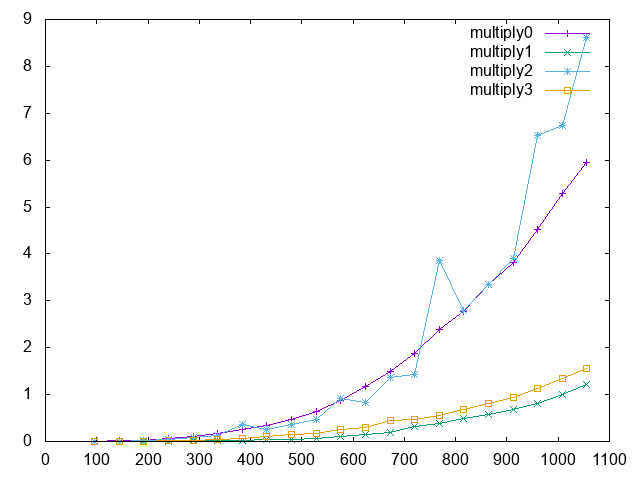
\includegraphics[scale=0.9]{matmult_res48.png}
 \captionof{figure}{Wykres przedstawiający czas mnożenia dwóch macierzy n x n w zależności od rozmiaru}

 Rozmiar kafelka ma wpływ na wydajność funkcji \texttt{multiply3}, jednak tylko w przypadku, gdy macierz jest odpowiednio duża.
 Poniżej możemy zobaczyć, że dla macierzy o rozmiarach mniejszych niż 1000x1000 różnica, choć jest obserwowalna, to nie jest znacząca.
 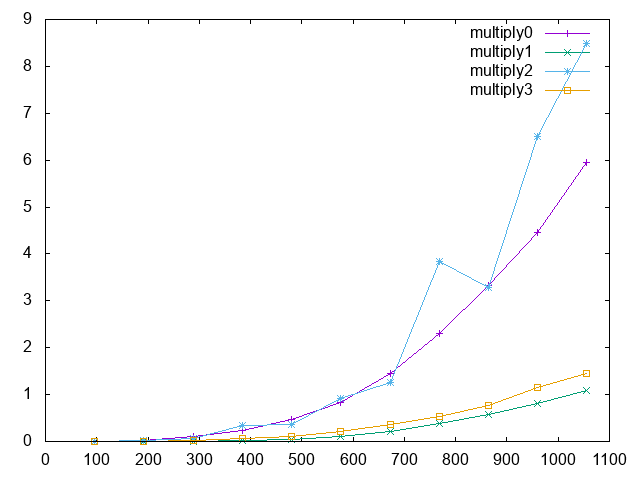
\includegraphics[scale=0.9]{matmult_4.png}
 \captionof{figure}{Wykres przedstawiający czas mnożenia dwóch macierzy n x n w zależności od rozmiaru przy kafelku rozmiaru 4 x 4}

 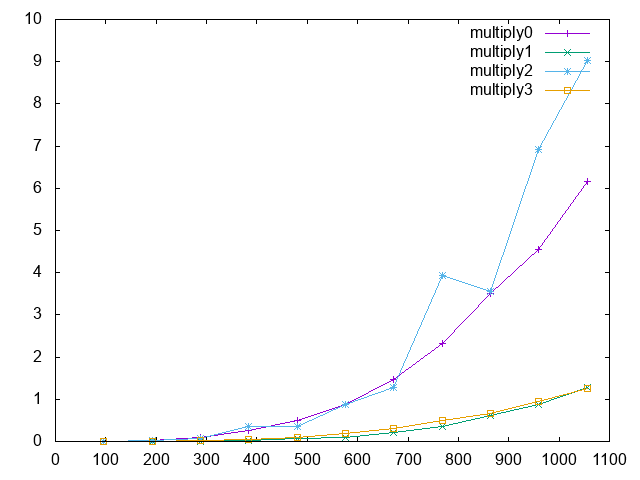
\includegraphics[scale=0.9]{matmult_8.png}
 \captionof{figure}{Wykres przedstawiający czas mnożenia dwóch macierzy n x n w zależności od rozmiaru przy kafelku rozmiaru 8 x 8}

 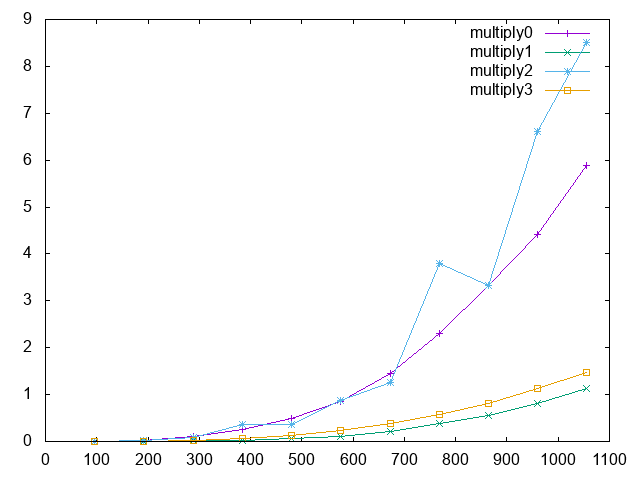
\includegraphics[scale=0.9]{matmult_res.png}
 \captionof{figure}{Wykres przedstawiający czas mnożenia dwóch macierzy n x n w zależności od rozmiaru przy kafelku rozmiaru 16 x 16, czyli domyślna wartość}

 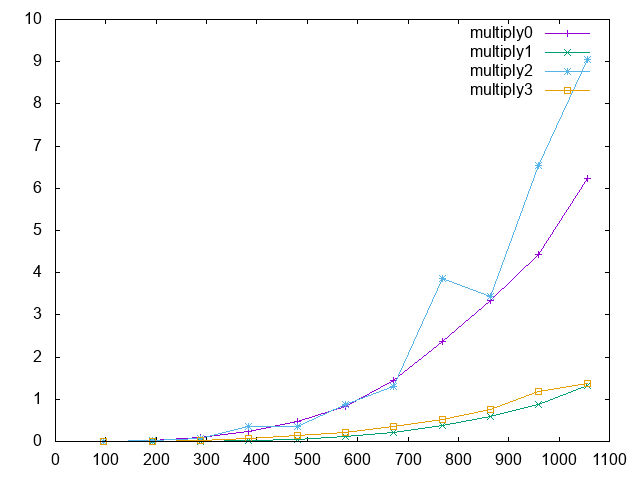
\includegraphics[scale=0.9]{matmult_32.png}
 \captionof{figure}{Wykres przedstawiający czas mnożenia dwóch macierzy n x n w zależności od rozmiaru przy kafelku rozmiaru 32 x 32}

 \section{Zadanie 3}
 Porównajmy najpierw nasze wyniki do tych przedstawionych na liście zadań.\footnote{W treść zadania przedstawionego na liście wkradł się mały błąd - tablica rozmiaru $2^{15}$ x $2^{15}$ przedstawiona na pierwotnej liście przy parametrze \texttt{-n 15} została wprost, oraz błędnie, przetłumaczona jako tablica o wymiarach 4096 x 4096, dlatego autor pozwolił sobie na zmianę tego parametru na bardziej przystępny.} \\
 \texttt{\$ ./transpose -n 16384 -v 0 \\
Generate matrix 16384 x 16384 (1048576 KiB) \\
Performing matrix transposition. \\
Time elapsed: 5.136787 seconds.\\}

\texttt{\$ ./transpose -n 16384 -v 1 \\
Generate matrix 16384 x 16384 (1048576 KiB) \\
Performing matrix transposition. \\
Time elapsed: 1.033438 seconds.\\}

 Udało nam się zoptymalizować nasz algorytm transpozycji macierzy wykorzystując metodę kafelkowania (dokładniej wykorzystując blok 8x8) i działa on około, przykładowo, sześciokrotnie szybciej dla macierzy rozmiarów 9728 x 9728 niż naiwna wersja o mniejszej lokalności.
 Pomiary dla kafelków rozmiaru 4x4, 8x8, 32x32 oraz 128x128.\\
 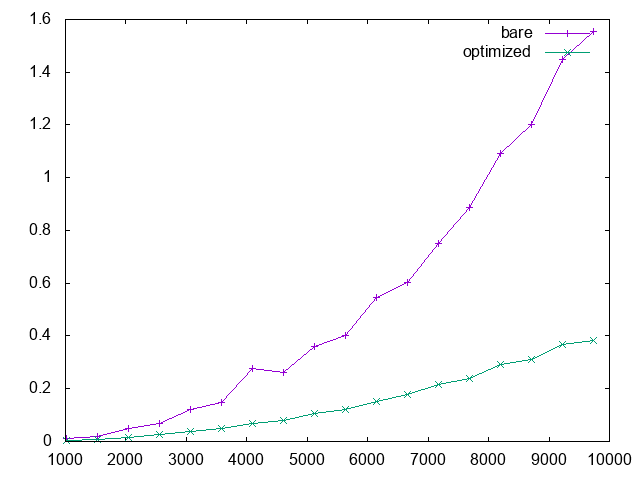
\includegraphics[scale=0.9]{transpose4.png}
 \captionof{figure}{Pomiary dla kafelka (bloku) rozmiaru 4.}
 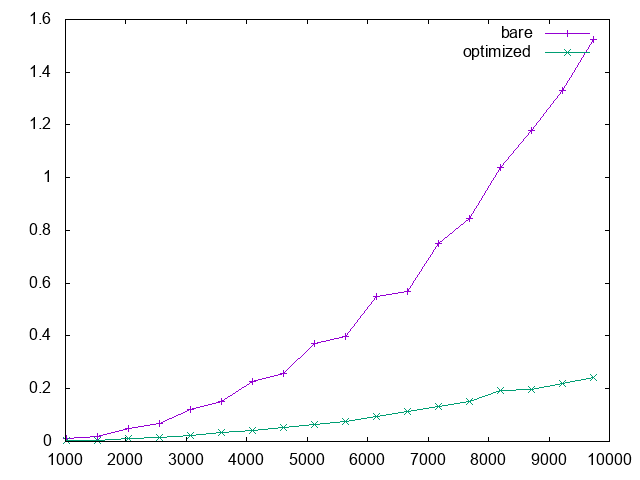
\includegraphics[scale=0.9]{transpose8.png}
 \captionof{figure}{Pomiary dla kafelka (bloku) rozmiaru 8, czyli wersja domyślna.}
 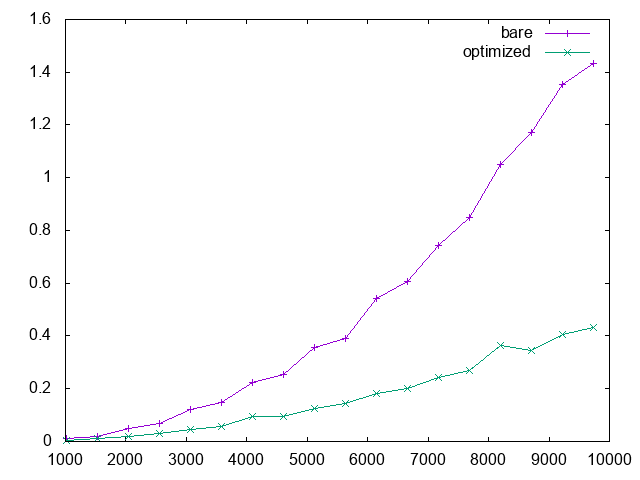
\includegraphics[scale=0.9]{transpose32.png}
 \captionof{figure}{Pomiary dla kafelka (bloku) rozmiaru 32.}
 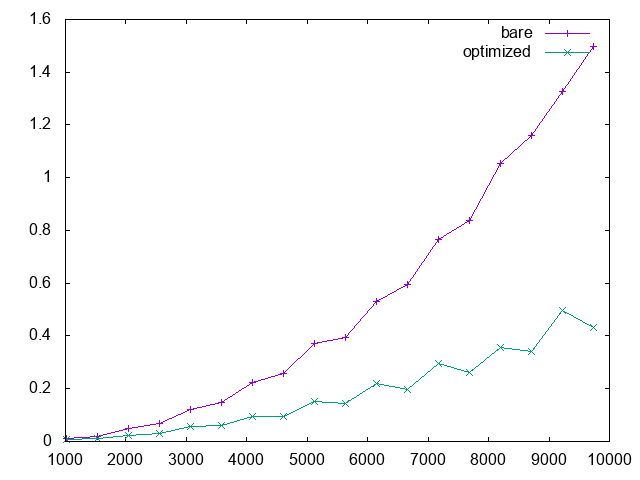
\includegraphics[scale=0.9]{transpose128.png}
 \captionof{figure}{Pomiary dla kafelka (bloku) rozmiaru 128.}
 Możemy na powyższych wykresach zauważyć, że rozmiar kafelka ma bardzo duże znaczenie dla czasu wykonania programu.
 Zdecydowanie najlepiej wypadła optymalizacja według domyślnego rozmiaru kafelka,
 czyli bloku rozmiaru 8 x 8, która była około 6 razy niż wersja niezoptymalizowana i około 2 razy szybsza niż wersje zoptymalizowane innymi rozmiarami bloków.
 Różnica między optymalizacją blokiem rozmiaru, czy to 4 x 4, czy 32 x 32, a blokiem 128 x 128 była niemal niezauważalna, z lekką przewagą bloku 4 x 4.

 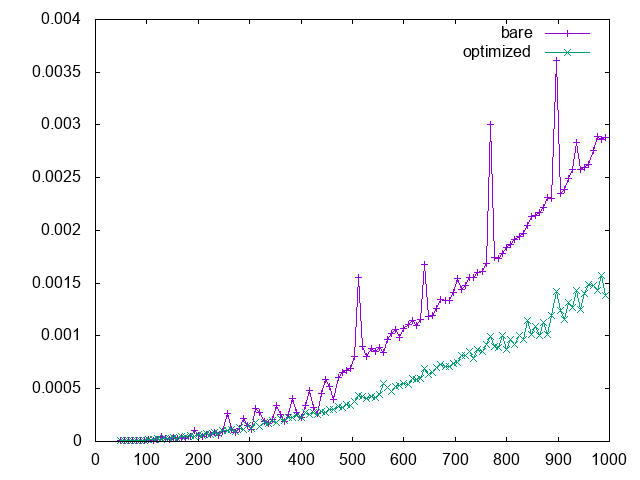
\includegraphics[scale=0.9]{transpose_cache.png}
 \captionof{figure}{Pomiary dla małych macierzy, w celu rozstrzygnięcia, czy można zidentyfikować rozmiary poziomów pamięci podręcznej}
 Możemy zauważyć skoki czasowe, chociażby, dla macierzy 256 x 256, 512 x 512, 640 x 640, 768 x 768 i 896 x 896, które są odpowiednio rozmiarów 1024 KiB, 1600 KiB, 2304 KiB oraz 3136 KiB.
 Dość nieprzewidzianym jest fakt, że przykładowo, macierz 520 x 520 transponowana jest szybciej, niż macierz 512 x 512 (nawet gdy testy te odpalimy manualnie, niezależnie od siebie oraz w różnej kolejności).
 Prawdopodobnie byłoby możliwe zidentyfikowanie rozmiarów poziomów pamięci cache, szczególnie widząc skok dla macierzy 896 x 896, która jest rozmiaru około 3MiB, czyli rozmiaru pamięci L3, oraz relatywnie duży skok dla macierzy 256 x 256 (256 KiB), czyli rozmiaru pamięci L2.
 Identyfikacja rozmiaru pamięci L1 (która jest rozmiaru 32 KiB) z taką metodą oraz obraną dokładnością raczej jest niemożliwa.
 Z drugiej strony bardzo prawdopodobne jest, że nawet maksymalne ograniczenie współbieżnie działających procesów nie pomaga przed procesami niezależnymi od użytkownika, co może zaburzać te wyniki.


 \section{Zadanie 4}
 Porównajmy najpierw nasze wyniki z tymi przedstawionymi na liście zadań. \\
 \texttt{
        \$ ./randwalk -S 0xea3495cc76b34acc -n 7 -s 16 -t 14 -v 0 \\
        Random number generator seed is 0xea3495cc76b34acc \\
        Generate matrix 128 x 128 (16 KiB) \\
        Performing 16384 random walks of 65536 steps. \\
        Time elapsed: 8.909246 seconds. \\
        Walks accrued elements worth: 3467540418 \\}

\texttt{
        \$ ./randwalk -S 0xea3495cc76b34acc -n 7 -s 16 -t 14 -v 1 \\
        Random number generator seed is 0xea3495cc76b34acc \\
        Generate matrix 128 x 128 (16 KiB) \\
        Performing 16384 random walks of 65536 steps. \\
        Time elapsed: 4.915772 seconds. \\
        Walks accrued elements worth: 3467540418 \\
}
Jak możemy przewidywać, nasza zoptymalizowana wersja funkcji \texttt{randwalk2} działa niemal 2 razy szybciej w porównaniu do poprzedniej wersji.
 Przed optymalizacją mieliśmy 152 instrukcje maszynowe, a po optymalizacji mamy 176 instrukcji maszynowych (sprawdzone przy pomocy \texttt{\$ objdump -d randwalk}),
 przy czym z 16 instrukcji postaci \texttt{Jcc} zamieniliśmy na dwie instrukcjie \texttt{Jcc} oraz 8 instrukcji \texttt{SETcc}
 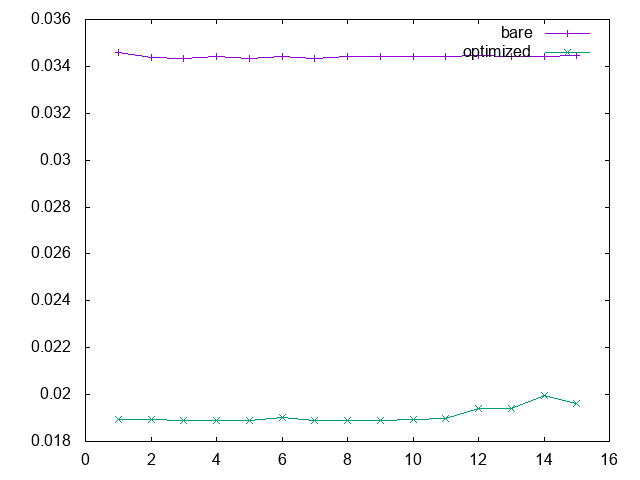
\includegraphics[scale=0.9]{randwalk_size.png}
 \captionof{figure}{Pomiary dla wywołań \texttt{\$ ./randwalk -S 0xea3495cc76b34acc -n X -s 12 -t 10 ...}}
 Możemy zaobserwować, że rozmiar tablicy nie ma zbytniego wpływu na czas działania programu.
 Ewentualnie ten czas może się w minimalnym stopniu wydłużyć,
 gdy tablica jest odpowiednio duża i nie mieści się w pamięci podręcznej procesora,
 przez co spada lokalność algorytmu, a dostępy do tablicy nieco wydłużają czas działania programu.
 Z drugiej strony warto zauważyć, że niezoptymalizowana wersja algorytmu również może cierpieć z tego powodu,
 lecz czas dostępów do tablicy jest ukryty pod karami za predykcję skoków w instrukcjach warunkowych.
 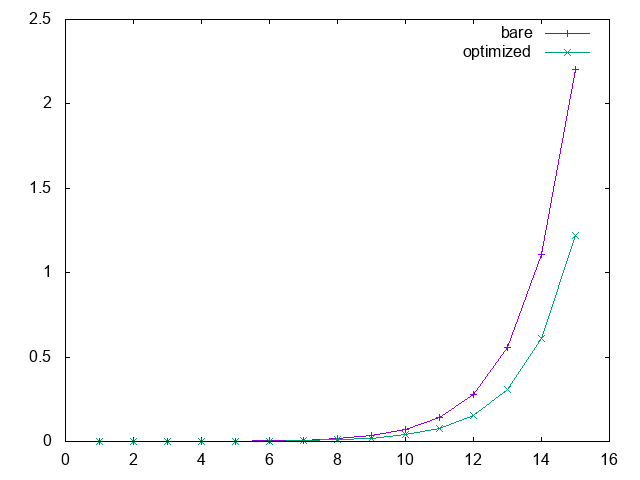
\includegraphics[scale=0.9]{randwalk_steps.png}
 \captionof{figure}{Pomiary dla wywołań \texttt{\$ ./randwalk -S 0xea3495cc76b34acc -n 14 -s X -t 13 ...}}
 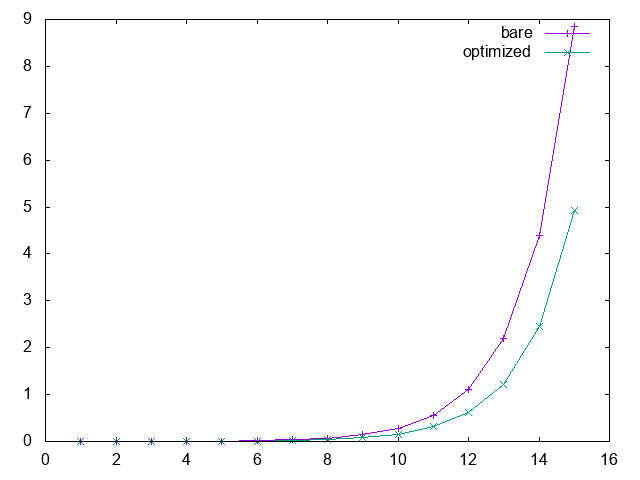
\includegraphics[scale=0.9]{randwalk_times.png}
 \captionof{figure}{Pomiary dla wywołań \texttt{\$ ./randwalk -S 0xea3495cc76b34acc -n 10 -s X -t 15 ...}}
 Na wykresach możemy zaobserwować około dwukrotne zmniejszenie czasu wykonania programu względem jego niezoptymalizowanej wersji.

 \section{Zadanie 5}
 Porównajmy najpierw nasze wyniki z tymi przedstawionymi na liście zadań. \\
 \texttt{
         \$ ./bsearch -S 0x5bab3de5da7882ff -n 23 -t 24 -v 0 \\
         Random number generator seed is 0x5bab3de5da7882ff \\
         Generate array of $2^{23}-1$ elements (32767 KiB) \\ % latex doesn't want to take 2^23 - 1 as a text :(
         Performing 16777216 searches \\
         Time elapsed: 11.195078 seconds. \\
         Number of searches that succeeded: 10610582/16777216 \\
         }

 \texttt{
         \$ ./bsearch -S 0x5bab3de5da7882ff -n 23 -t 24 -v 1 \\
         Random number generator seed is 0x5bab3de5da7882ff \\
         Generate array of $2^{23}-1$ elements (32767 KiB) \\
         Performing 16777216 searches \\
         Time elapsed: 4.037533 seconds.\\
         Number of searches that succeeded: 10610582/16777216 \\
 }
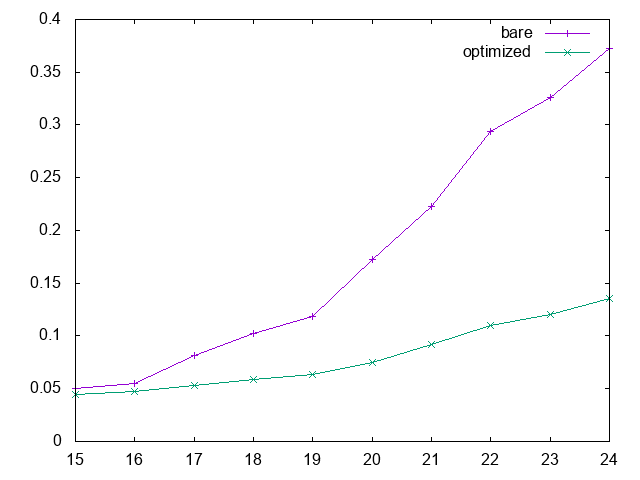
\includegraphics[scale=0.9]{bsearch_res.png}
\captionof{figure}{Pomiary dla wywołań \texttt{\$ ./bsearch -S 0x5bab3de5da7882ff -n X -t 19 ...}}
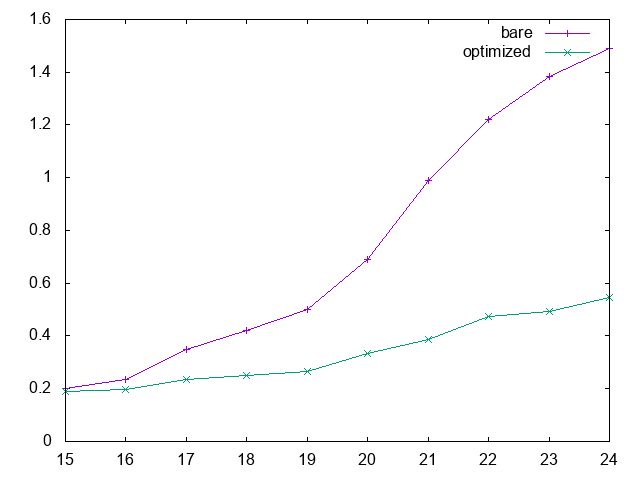
\includegraphics[scale=0.9]{bsearch_res21.png}
\captionof{figure}{Pomiary dla wywołań \texttt{\$ ./bsearch -S 0x5bab3de5da7882ff -n X -t 21 ...}}


 Zmiana organizacji danych spowodowała przyspieszenie algorytmu, ponieważ w strukturze kopcowej, wszystkie elementy są posortowane według użyteczności. Innymi słowy, wiemy, że zdecydowanie
 bardziej prawdopodobnym będzie odwoływanie się do elementów dzielących naszą wejściową tablicę na mniejsze połówki w wyszukiwaniu binarnym, które
 w tablicy reprezentującej kopiec są ustawione spójnymi blokami (tj. kopiec jest ułożony poziomami),
 a zdecydowanie rzadziej potrzebujemy elementów ukrytych pod liśćmi w naszym kopcu, czyli tych na samym końcu kopca. W ten sposób zwiększyliśmy hit-rate.
 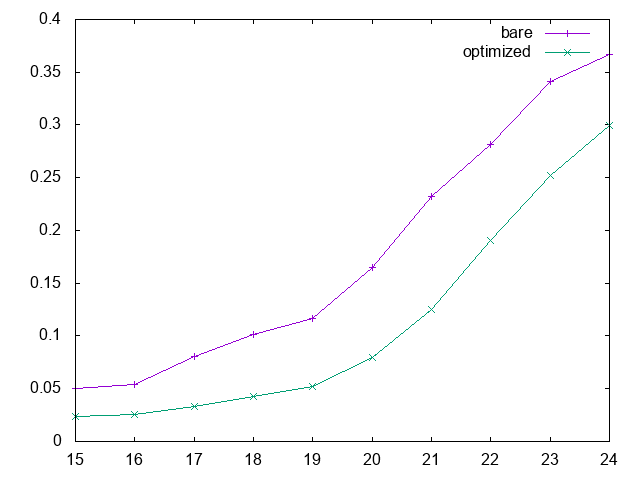
\includegraphics[scale=0.9]{bsearch_if1.png}
 \captionof{figure}{Pomiary dla wywołań \texttt{\$ ./bsearch -S 0x5bab3de5da7882ff -n X -t 19 ...}, gdy sprawdzenie, czy znaleźliśmy dany element zostawimy na koniec pętli.}

 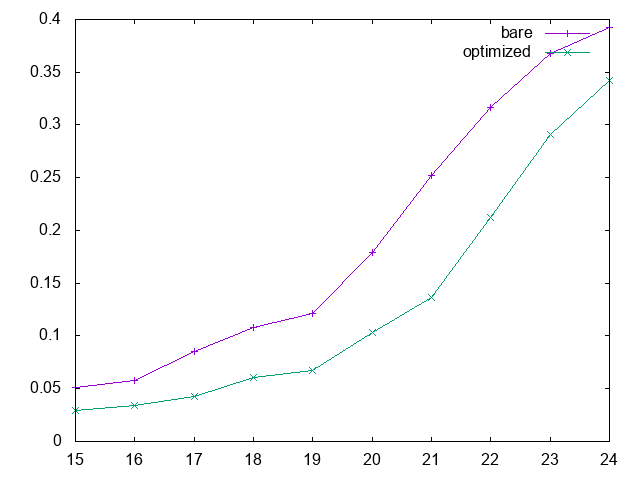
\includegraphics[scale=0.9]{bsearch_if2.png}
 \captionof{figure}{Pomiary dla wywołań \texttt{\$ ./bsearch -S 0x5bab3de5da7882ff -n X -t 19 ...}, gdy zastąpimy linie 54-55 na jedno przypisanie do zmiennej \texttt{i}.}

Odpowiednie ułożenie instrukcji w ciele \texttt{heap\_search} mocno wpływa na wydajność programu.
Przykładowo, przesunięcie linii 51 - 52 (czyli instrukcji warunkowej sprawdzającej czy znaleźliśmy dany element) na sam koniec pętli (między linie 58 i 59) powoduje niemal dwukrotne wydłużenie działania programu względem zoptymalizowanego.
Paradoksalnie też, zastąpienie instrukcji przypisania do \texttt{i} w liniach (54-55) odpowiadających za decyzję, którego syna w danego wierzchołka wybrać, na fragment \texttt{i = (i << 1) + 1 + !(y > x)} również bardzo mocno wydłuża czas działania programu,
natomiast nie obserwujemy takiego spowolnienia, gdy linijkę 55 rozbijemy na wyrażenie warunkowe \texttt{if}.
\end{document}
